\documentclass[11pt,twoside]{report}
\usepackage{preamble}
\graphicspath{{../img/ch6/}}
\setcounter{chapter}{5}

\begin{document}

\chapter{Modelling Zebrafish}
\label{chapter:fish_model}


\epigraph{人相忘乎道术}{庄子}


\section{Introduction}

In this chapter we will study the behaviour of the zebrafish with the help of computer simulation. The goal of the simulation is to reproduce the experimental results from chapter~\ref{chapter:fish_2d} to chapter~\ref{chapter:fish_analysis}.
We will use the Monte-Carlo simulation to study a system in equilibrium, in order to reproduce the spatial distribution of the fish under the influence of the boundary, the gravity, as well as the pairwise interaction.
In addition, we will use a dynamical simulation to study an agent-based\marginfootnote{
The dynamical simulation is similar to the Brownian dynamics simulation for the liquid, where all the particles were updated according the force exerted on them. It's different from the Monte-Carlo simulation where the particles are moved randomly.
The moving individuals in the model can take different names, like the ``particles'', ``animals'', and ``agents''. The term ``agents'' will be used in this chapter for consistency.
} active matter model, in order to recreate the dynamical feature of the fish group in the experiments.
%The purpose of these simulations is to understand and explain the observed zebrafish behaviour, so that we could get more insights into its nature. 
%In particular we focus on the distribution of the density, as well as the order of the dynamics.

The density distribution of the fish was strongly affected by the presence of the boundary, as the fish were physically constrained in the tank.
For the 3D experiment, the distribution of the fish was also affected by an ``effective gravity'', as well as the holes drilled on the tank. These environmental factors can be treated as external fields affecting the fish. In addition to these external factors, the fish-fish interaction will also change their distribution.
With the Monte-Carlo (\gls{MC}) simulation techniques, we can study these effects individually. Using such simulation method, we assumes the fish group were in equilibrium. Such assumption is not valid since a group of fish is an active matter system. By applying this invalid assuption, we implicitly tested the idea of mapping active matter system to an equilibrium counterpart, where the non-equilibrium feature of the system, the activity, was summarised by an effective temperature\marginfootnote{
This ``effective equilibrium'' picture is supported by the exponential decay of the excess distribution function shown in section~\ref{section:fish_1_3d}, as the decay suggests the Boltzmann-like distribution commonly seen in equilibrated systems.
} \cite{palacci2010, klongvessa2019}. The MC approach ignores the dynamics of the system, but will give us insights regarding the structure (density distribution) of the fish group.

For a group of fish, the order of their dynamics, captured by the polarisation value (Eq.~\ref{eq:polarisation}), correlates robustly with a non-dimensional value \gls{kappa}, the ratio between the persistence length (\gls{lp}) and the nearest neighbour distance (\gls{lnn}).
Such a correlation suggests the local density and the persistence motion of the fish dominated the polarisation of the system.
Since the persistence motion is a proxy to the \emph{activity} of the fish, the entire group of 50 zebrafish is behaving like an alignment dominated active matter system (section~\ref{section:active-phase}).
To confirm the similarity of a group of zebrafish, and a model active matter system, we will use the dynamical simulation method to simulate the famous active matter model, the Vicsek model \cite{vicsek1995}.
Such simulation ignores the structure of the fish group, where all the structural features are absorbed into the number density parameter in the model (section~\ref{section:vicsek-model}).
To get a good fit between the model and the experiments, we will have to modify the Vicsek mode and consider the orientational inertia of the fish.
The fitting of the model and the experimental result suggests the existence of the effective alignment interaction among the fish. And the changing states of the fish could be understood as a change of the noise level for the model.


\section{Simulation Methods}


\subsection{General Idea}

If we think of fish as a collection of agents following pre-defined movement rules, we could reproduce the movement of the fish with the computer simulation. Formally, we call a collection of agents a \emph{system}. And the system can change its (microscopic) states over time.
By observing the system for a long time, we could obtain the trajectory of the system, and then calculate the quantities that we are interested in (see chapter~\ref{chapter:fish_analysis} for examples). Such process is summarised in the following algorithm (Algorithm~\ref{alg:simulation}).
During the simulation, the system change its states under some constraints. For example, the constraints could be a controlled noise level (\gls{beta}), a constant number density (\gls{rho}), and a fixed total number (\gls{N}) of agents.


\begin{algorithm}
	\KwData{Constraints $\{ \beta, \rho, N, \dots \}$}
	\KwResult{Trajectory}
	System $\gets$ initial microscopic state with $\{ \beta, \rho, N, \dots \}$\;
	\Repeat{System is stable, and forgets the initial microscopic state}{
		change the microscopic state of the system with $\{ \beta, \rho, N, \dots \}$
	}
	Trajectory $\gets \emptyset$\;
	\Repeat{
		The statistics are good enough
	} {
		change the microscopic state of the system with $\{ \beta, \rho, N, \dots \}$\;
		Put current state in Trajectory\;
	}
\caption{The Simulation Procedure}
\label{alg:simulation}
\end{algorithm}

\subsection{Monte-Carlo Simulation}

There are multiple ways to change the state of the system in algorithm~\ref{alg:simulation}. In a seemly arbitrary fashion, we could change the state of the system randomly, and reject some states that is unlikely to happen. This method is termed ``Monte-Carlo'' (MC) simulation, and the acceptance ratio were often determined by the Metropolis algorithm.
Typically, the acceptance ratio from state $\zeta$ to $\nu$, \gls{acc}, is written as

\[
	A(\zeta \rightarrow \nu) = \left\{
		\begin{array}{ll}
			\exp\left(-\beta(E_\nu - E_\zeta)\right)
			& \mbox{if $E_\nu - E_\zeta > 0$}\\
			1 & \mbox{otherwise.}
		\end{array}
	\right.
\]

\noindent And the values of $E_\nu$ and $E_\zeta$ represent the energy values of state $\nu$ and $\zeta$, respectively. The value $\beta$ is the inverse temperature. The smaller $\beta$ value is, the higher the temperature, and the larger randomness the system exhibits. Sampling the states with this acceptance ratio, we are effective sampling an equilibrium system, whose states follow the Boltzmann distribution. For a microscopic state $\nu$, its probability to be sampled is $\exp(-\beta E_\nu) / Z$, were $Z$ is a normalisation factor (the partition function).

With MC simulation, it is easy to constrain the agents in the fish tank, by setting $E = \infty$ once an agent is outside the tank.\marginfootnote{
Operationally, we reject the states if any agent is outside the fish tank.
} In addition, the effect of external fields, like gravity, can be added easily to the simulation. However, due to the lack of ``true'' dynamics in the MC simulation, we will not have access to the velocities of the system. Hence, this simulation method is only used to model the spatial distribution of the zebrafish.


\subsection{Dynamical Simulation}


Another way to change the state of the system is to integrate the \emph{equation of motion} of all the agents. For animals, the equations to be integrated represent the behavioural rules of the agents.
Being different from the conventional molecular dynamics simulation or mesoscale simulations \cite{allen2017}, the simulation of animal behaviour often incorporates more eccentric rules, such as a fixed vision zone\cite{couzin2002, yigit2020}, and an attraction to the group centre \cite{reynolds1987}. Generally, the updating rules for the agents could be described by the following equation,

\begin{equation*}
\begin{split}
	\mathbf{v}_{i}^{t+1}
	&= \mathcal{B} [\mathbf{v}_{i}^t] \\
	\mathbf{x}_i^{t+1}
	&= \mathbf{x}_i^{t} + \mathbf{v}_i^{t+1},
\end{split}
\end{equation*}

\noindent where the operator $\mathcal{B}$ encodes all the behavioural rules of the animals. By changing the coordinates and velocities of all the agents simultaneously, we change the state of the system (Algorithm~\ref{alg:simulation}).


\section{The Distribution of the Density}
\label{section:simulate-density}

In this section we will model the spatial distribution of the fish in the 3D experiment. The simulation will illuminate the effects of the environmental factors, such as the fish tank and the gravity. By comparing with the experimental density distribution, we can get phenomenological parameters such as the effective temperature, to describe the behaviour of the fish.



\subsection{The Effect of the Tank}
\label{section:sim-mc-tank}

The 3D geometry of the tank confining the zebrafish was determined in section \ref{section:system_3d}, and the shape of the tank can be expressed as,

\begin{equation*}
	z = c r^2,	
\end{equation*}


\noindent where $c=0.74 m^{-1}$ when both $r$ and $z$ were expressed in the unit of meters. The volume (\gls{vol}) of the tank can be calculated as

\begin{equation*}
	V = \int_{0}^{h}{\pi \frac{z}{c}} dz
	  = \frac{\pi h^2}{2 c},	
\end{equation*}


\noindent where $h$ is the height of the tank, the vertical distance between the water surface and the base of the tank. The joint probability density function (PDF) of random points, being uniformly distributed inside the tank, is written as,

\begin{equation*}
	f(x, y, z) = V^{-1} = \frac{2c}{\pi h^2}.		
\end{equation*}

\noindent The joint PDF of the uniform distribution can be expressed in the spherical coordinates as,

\begin{equation}
	f(\theta, r, z) = \frac{2c}{\pi h^2} r,
\label{eq:density-pdf-tank}
\end{equation}

\noindent where $\theta$ is the azimuthal angle, $r = \sqrt{x^2 + y^2}$ is the radius in $XY$ plane.  From the expressions above, we can calculate the marginal distribution of $r$ and $z$ coordinates:

\begin{equation}
\begin{split}
	f_R(r) &= \int_0^{2\pi}{d \theta} \int_{cr^2}^{h}{dz} \; f(\theta, r, z)
		= \frac{4c}{h} r - \frac{4 c^2}{h^2} r^3, \\[2em]
	f_Z(z) &= \int_0^{2\pi}{d \theta} \int_0^{\sqrt{z/c}}{dr} \; f(\theta, r, z) 
	= \frac{2}{h^2} z.
\end{split}
\label{eq:dist-tank}
\end{equation}

\noindent The analytical result (Eq.~\ref{eq:dist-tank}) is checked against the numerical sampling of random points inside the tank, as shown in Fig.~\ref{fig:dist-tank}. These PDFs can be used as comparison for the distribution of real fish data, as presented in section~\ref{section:observe-3d-result}. The experimental distribution of the fish is very different from the ideal gas distribution.

\begin{SCfigure}
  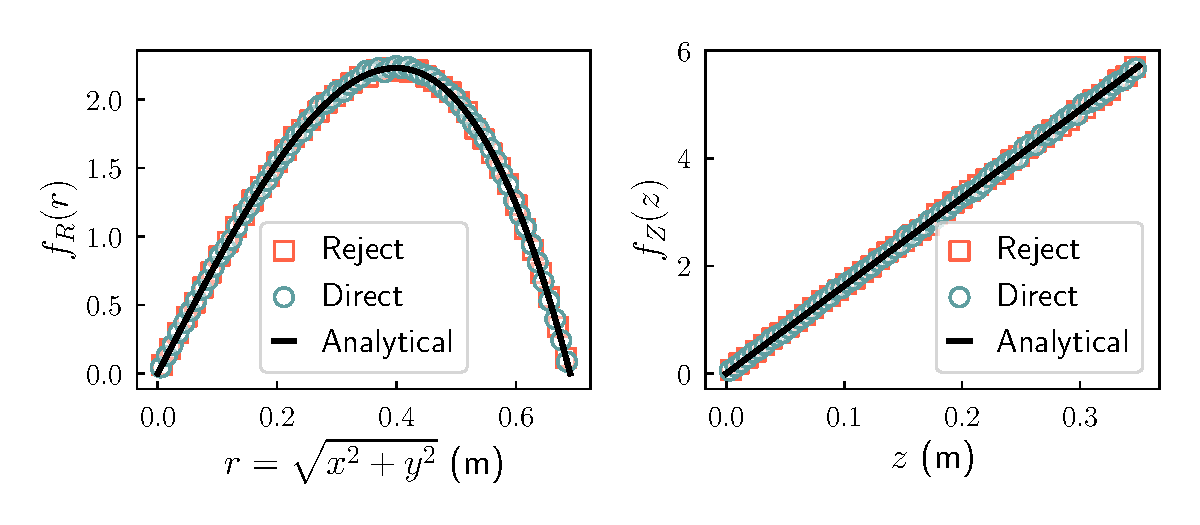
\includegraphics[width=\linewidth]{density-tank}
  \caption[The 3D geometry of the experimental fish tank]{
  The marginal probability density distribution of points sampled uniformly inside the experimental fish tank.
  Left: the distribution the planar radius $r$.
  Right: the distribution of the $z$ component of the points.
  }
  \label{fig:dist-tank}
\end{SCfigure}


\subsection{The Effect of the ``Gravity''}
\label{section:sim-mc-gravity}

\begin{SCfigure}
  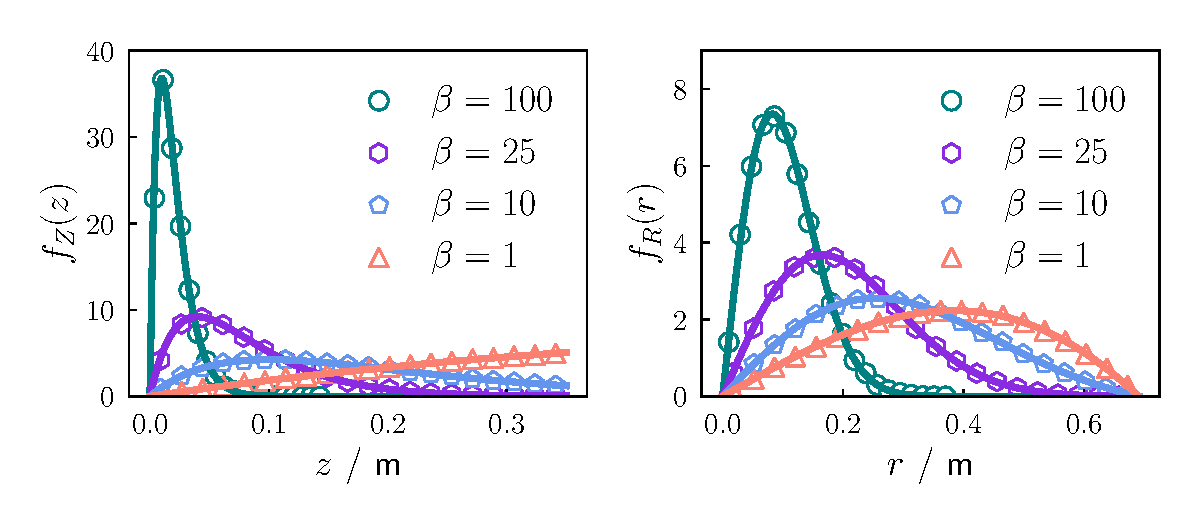
\includegraphics[width=\linewidth]{density-gravity}
  \caption[The distribution of ideal gas in the tank subjected to gravity]{The marginal probability density distribution of ideal gas particles sampled uniformly inside the experimental fish tank, where the particles were subjected to the gravity field. Left: the distribution the $z$ component. Right: the distribution of the $r = \sqrt{x^2 + y^2}$. The scatters were result of Monte-Carlo simulations, and the solid lines were from Eq.~\ref{eq:dist-gravity}.}
  \label{fig:dist-gravity}
\end{SCfigure}

From the results presented in section~\ref{section:observe-3d-result}, it is evident that the zebrafish will be affected by an ``effective gravity'', because of their depth preference behaviour.
This effective gravity is similar to 
As a first attempt, we could calculate the density distribution of ideal gas particles in equilibrium, with an Boltzmann weight $\exp(-\beta z)$ to capture the effect of the gravity.
The \emph{partition function} (\gls{Z}) of the system is written as,

\begin{equation*}
	Z = \int_0^h \pi \frac{z}{c} \exp(-\beta z) dz
      = \frac{\pi (1 - \exp(-\beta h) (1 + \beta h))}{c \beta^2}.
\end{equation*}

\noindent With the partition function, we could then calculate the joint probability density function of the ideal gas, in the spherical coordinate system (similar to Eq.~\ref{eq:density-pdf-tank}).

\begin{equation}
	f(\theta, r, z)
	= \frac{r \exp(-\beta z)}{Z}
	= \frac{c \exp(-\beta z) r \beta^2}
	{\pi(1 - \exp(-\beta h)(1 + \beta h))}
\label{eq:density-pdf-gravity}
\end{equation}

\noindent where $\beta = 1 / (k_B T)$ is the inverse temperature. For a physical systems in equilibrium, the vale of \gls{beta} relates to the real temperature measured by a thermometer. However, the value of $\beta$ for the fish only controls the level of randomness of the system, without a concrete physical meaning. From the function $f(\theta, r, z)$, we can calculate the distribution functions $f_R(r)$ and $f_Z(z)$:

\begin{equation}
\begin{split}
	f_R(r) &= \int_0^{2\pi}{d \theta} \int_{cr^2}^{h}{dz} \; f(\theta, r, z)
		= \frac{
			2 c \left(
					\exp \left( \beta (h - c r^2) \right) - 1
				\right) r \beta
		}{
			\exp(\beta h) - \beta h - 1
		}, \\[2em]
	f_Z(z) &= \int_0^{2\pi}{d \theta} \int_0^{\sqrt{z/c}}{dr} \; f(\theta, r, z) 
	= \frac{\exp(-z \beta) z \beta^2}{
		1 - \exp(-\beta h) (1 + \beta h)
	}.
\end{split}
\label{eq:dist-gravity}
\end{equation}

\noindent The results from Eq.~\ref{eq:dist-gravity} were checked against the Monte-Carlo simulation results, as shown in Fig.~\ref{fig:dist-gravity}. With the increase of $\beta$, hence the decrease of temperature, the agents were pushed towards smaller $z$ values and $r$ values. By ``fitting'' the experimental results with the analytical results from Eq.~\ref{eq:dist-gravity}, and setting $\beta$ as a free parameter, we could obtain the effective temperature for the fish.
%A systematic study of the change of the effective temperature could give us a more systematic understanding of the depth preference of the zebrafish. For instance, the fitting parameter $\beta$ could be interpreted as the ``fear'' perceived by the fish.




\subsection{The Effect of the Holes}
\label{section:sim-mc-holes}

In our 3D fish observation experiments, the holes on the tank disrupted the density distribution of the fish. This disruption makes the result in Eq.~\ref{eq:dist-gravity} very different from the distribution of the fish, as shown in section~\ref{section:holes}. To mimic such effect, we could model holes as an extra field, with the following form,

\begin{equation}
	H(r, z) = q
		\sum_i{\frac{
		\left[
			(r - r_i)^2 + (z - c r_i^2)^2
		\right]^{-2}
		}{r_i}},
\label{eq:energy-holes}
\end{equation}

\noindent where $r_i$ represents the location of the holes on the tank. Specifically, there are three sets of holes (Fig.~\ref{fig:density-holes}), located at $r_1=96$ mm, $r_2=213$, and $r_3=327$ mm. The denominator ($r_i$) in Eq.~\ref{eq:energy-holes} represents the fact that equal amount of holes were drilled on the circles. So that the larger circles will have less holes per unit length. The factor \gls{q} controls the strength of the repelling interaction between the fish and the holes.

Calculating the corresponding density distributions, \gls{pdfr} and \gls{pdfz}, analytically is difficult, but we can estimate the density distribution with the Monte-Carlo simulation. Figure~\ref{fig:dist-holes} shows the result of the simulation. As expected, the distribution $f_R(r)$ appears bimodal with a locally minimum $q$ value at the location $r = r_1$.

\begin{SCfigure}
  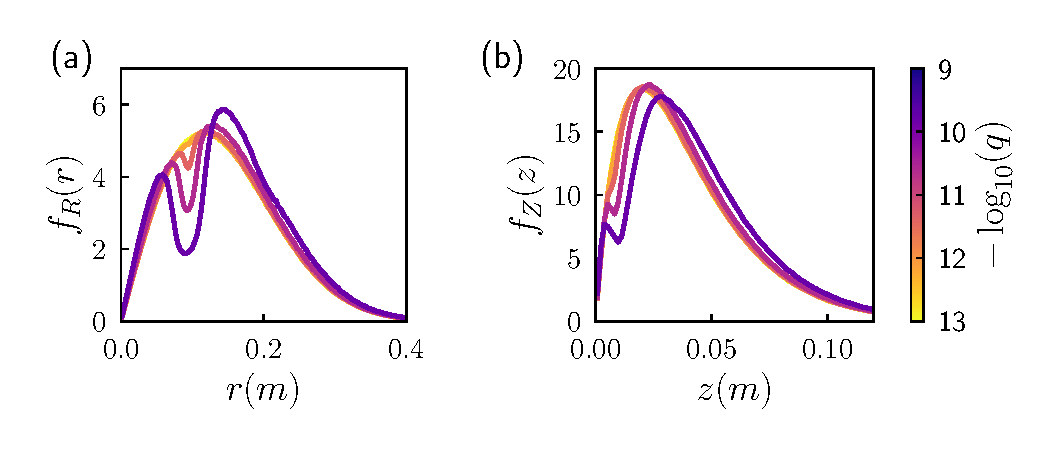
\includegraphics[width=\linewidth]{density-holes}
  \caption[The effect of the holes on the density distribution]{
  The effect of the holes on the density distribution of ideal gas in the fish tank subjected to gravity field.
  (a): the distribution the $z$.
  (b): the distribution of the $r$.
  The colour of the lines indicates the strength of the repulsive interaction of the holes on the tank. The simulation was carried out with parameter $\beta=50$, where $7.5 \times 10^{6}$ coordinates were sampled.
  }
  \label{fig:dist-holes}
\end{SCfigure}


\subsection{The Effect of Pairwise Interaction}
\label{section:sim-mc-interaction}


\marginpar{
\centering
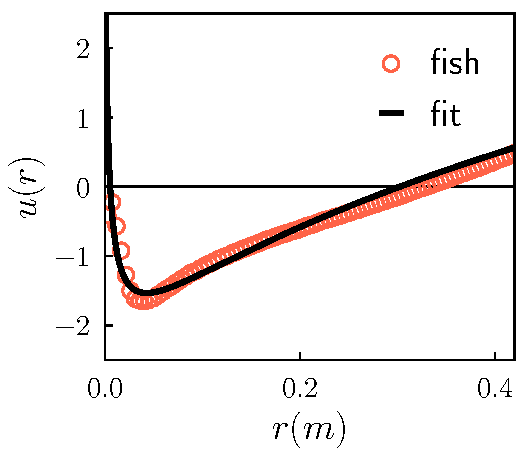
\includegraphics[width=\marginparwidth]{fit-gr}
\captionof{figure}{Fitting the $u(r)$ of fish with Eq.~\ref{eq:fit-ur}.}
\label{fig:fit-ur}
}

The simulations in section~\ref{section:sim-mc-tank} to \ref{section:sim-mc-holes} treat the agents as ideal gas particles, without any interaction between the agents. This is not realistic, since the $g(r)$ of the zebrafish exhibits characteristic features (Fig.~\ref{fig:structure-3d} (c) in section~\ref{section:analysis-structure-3d}).
In order to enable the agents to behave more like the zebrafish in the simulation, we added an effective interaction among the agents. We assume the interaction is pairwise, and spherically symmetrical, therefore ignored the possible many-body interactions \cite{kursten2020}.

To implement the pairwise interaction in the Monte-Carlo simulation, we assign the effective potential energy\marginfootnote{
Notice the logarithm of $g(r)$ is $-\beta u(r)$ for equilibrium systems. Here we ignored the $\beta$, and we controlled the strength of the pairwise interaction with parameter $q$.
The reason for our choice is that we are only interested in the approximated shape of $u(r)$, which makes the fish forming a coherent group.
}, \gls{ur}, for all the pairs of agents. The potential energy is written as,

\begin{equation*}
	u(r) = -p \log\left[ g(r) \right]
\end{equation*}

\noindent where \gls{p} is a free parameter that determines the contribution of the interaction between the agents. To parameterise the experimental $u(r)$, we fitted it with function

\begin{equation}
	u(r) = \log(a_1) - \log(2)\left[
		\frac{
			\log(1 + 2a_2(r-a_3)/a_4)
		}{a_2}
	\right]^2,
\label{eq:fit-ur}
\end{equation}


\noindent where $a_1$ - $a_4$ are fitting parameters. Figure~\ref{fig:fit-ur} shows the fitting result, where the potential energy took a minimum at the location of nearest neighbour distance.
We can incorporate this pairwise interaction into the energy form during the Monte-Carlo simulation, to study its effects. Formally, the energy of the system could be written as,


\begin{equation}
	E = \left\{ \begin{array}{ll}
		\sum_i\left[
			z_i + H(r_i, z_i) + 
			\sum_{j \neq i}{u(d_{ij})} 
			\right]
			&  \mbox{if $c r_i \le z_i < h$}\\
		\infty & \mbox{otherwise}
	\end{array}\right.
\label{eq:model-density}
\end{equation}



\noindent where the coordinate of agent $i$ is $(x_i, y_i, z_i)^\top$, with $r_i = \sqrt{x_i^2 + y_i^2}$. The condition ($c r_i \le z_i < h$) ensures the agents staying in the boundary. This ``energy'' is a mixture of the effective gravity\marginfootnote{
Notice we implicitly transformed the height of the fish ($z_i$) to the potential energy in an effective gravitational field in Eq.~\ref{eq:model-density}.
}, the repulsive holes, and the pairwise interaction, and it is controlled by parameter $p$ and $q$.
When both $p$ and $q$ are equal to zero, the agents behave like ideal gas in the tank subjected to the effective gravity. But tuning the value of $p$ and $q$, we increase the effect of the pairwise interaction and the holes.

\begin{SCfigure}
  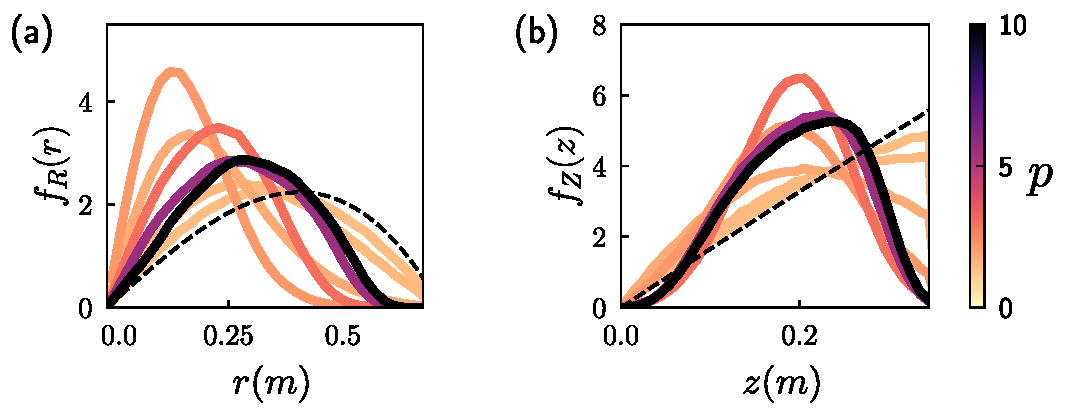
\includegraphics[width=\linewidth]{density-interaction}
  \caption[The effect of the pairwise interaction on the density distribution]{
  The effect of the pairwise interaction among the agents, on their density distribution.
  (a): the distribution the planner radius $r=\sqrt{x^2 + y^2}$ of the agents' coordinates.
  (b): the distribution of the $z$ component of the agents' coordinates.
  The colour of the solid lines indicates the strength of the pairwise interaction of the fish. The dashed lines corresponds to the result where $p=0$. The simulation was carried out with parameter $\beta=0.1$, where $5 \times 10^{5}$ coordinates were sampled.
  }
  \label{fig:dist-interaction}
\end{SCfigure}

The effect of the pairwise interaction of the fish on the density distribution is shown in Fig.~\ref{fig:dist-interaction}, where we fixed the value of $q$ (which controls the strength of the fish-hole interaction) to be $0$, and set $\beta=0.1$. These parameters correspond to the condition where the effects of both the gravity and the holes could be ignored.
When the value of $p$ is small, so that the interaction among the agents are weak, the system behaves like ideal gas particles under gravity, described by Eq.~\ref{fig:dist-interaction}. When the value of $p$ was gradually increased from $10^{-2}$ to 1, the fish tend to aggregate near the bottom of the tank in the centre.

\marginpar{
\centering
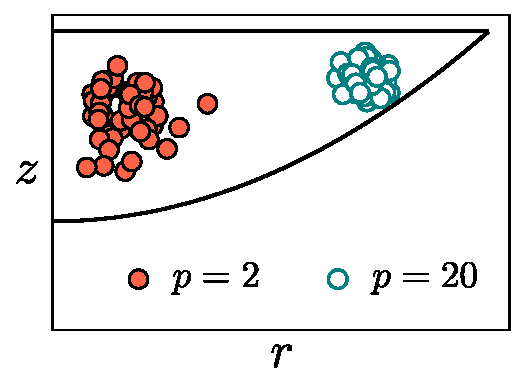
\includegraphics[width=\marginparwidth]{fish-cluster}
\captionof{figure}{The parameter $p$ controls the size of the group.}
\label{fig:fish-cluster}
}



Notably, the further increase of $p$ would change the density distribution of the fish in a different fashion. As the value of $p$ increased from 1 to 10, the fish are more frequently appear at higher $r$ and $z$ values. Such non-monotonic behaviour could be understood by carefully examining the effective interaction potential $u(r)$ of the agents.
Typically, the interaction potential would constrain the agents to form a coherent cluster, to mimic the observed structure of the fish group (section~\ref{section:analysis-structure-3d}). And the size of the cluster would decrease, with the increase of $p$, as shown in Fig.~\ref{fig:fish-cluster}.
For smaller clusters, they would be able to explore the ``corner'' of the fish tank, where both $r$ value and $z$ value are high.
On the other hand, the large clusters would have to deform its shape, paying extra energy cost, so that they could enter the corner region.
Therefore, the agents with stronger pairwise interaction would explore more space in the tank, presenting higher chance to appear in regions where $r$ and $z$ values are high.





\subsection{Comparison to Experimental Data}

\begin{SCfigure}
  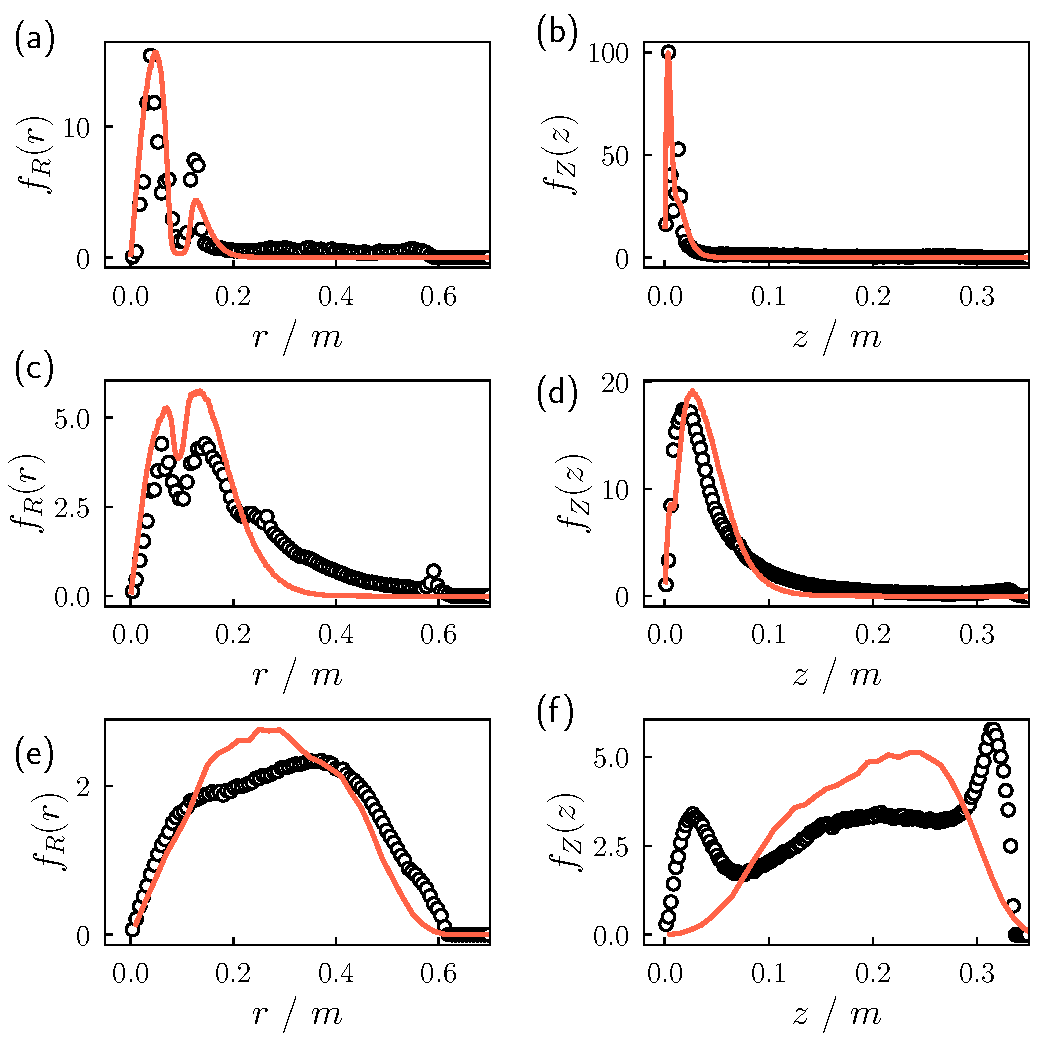
\includegraphics[width=0.9\linewidth]{model-density}
  \caption[Comparing the density distribution of the fish and the model]{
  The comparison of the density distribution of fish with the model described by Eq.~\ref{eq:model-density}. The data points represent the experiment measurements, and the solid lines were calculated from the Monte-Carlo simulation.
  (a): the distribution the $z$ from 1 fish.
  (b): the distribution of the $r$ from 1 fish.
  (c): the distribution the $z$ from 2 fish.
  (d): the distribution of the $r$ from 2 fish.
  (e): the distribution the $z$ from 50 fish.
  (f): the distribution of the $r$ from 50 fish.
  }
  \label{fig:model-density}
\end{SCfigure}

We used the energy term in Eq.~\ref{eq:model-density} to simulate the equilibrium density profile of the agents, and compare the results with our experimental data obtained in chapter~\ref{chapter:fish_3d}. By tuning the parameters, typically the values of $\beta$, $q$, and $p$ manually, we can generated simulation result that is similar to the experimental results. The fitting result is shown in Fig.~\ref{fig:model-density}.

For the distribution of one fish in the tank, the fitting results suggests an effective inverse temperature of $\beta = 200$, and the strength of the fish-hole interaction of $a = 2\times 10^{-10}$, as presented in Fig.~\ref{fig:model-density} (a) and (b). By decreasing the value of $\beta$ to 45, and incorporating the fish-fish interaction with $p = 10$, we could model the density profile of 2 fish, as shown in Fig.~\ref{fig:model-density} (c) and (d). There is a slight mismatch between the experiment and the model, which might related to the non-equilibrium nature of the fish, which is absent in our Monte-Carlo simulation.
 
 To match the density profile of 50 fish, the value of $\beta$ needs to be further decreased to 0.1, while keeping the $q$ and $p$ values unchanged. However, the match between the experimental data and the model is poor. In fact, the bimodal distribution of $f_Z(z)$ of 50 fish, shown in Fig.~\ref{fig:model-density} (f), indicates the presence of multiple states, as reported in section~\ref{section:change-states-3d}. To take multiple states into consideration, we will need to overlay simulation results from multiple systems with different parameters. Such a complex simulation is beyond the scope of this chapter.
  
Even though the fitting between the experimental density distribution and that from the Monte-Carlo simulation is not very good, the result is in accordance with our previous discussion in chapter~\ref{chapter:fish_2d} and \ref{chapter:fish_3d}. Namely, when the number of fish is small, the interaction between the fish and the environment (gravity and holes) is significant. Such importance could be translated to a high $\beta$ value in our model. For a group of 50 fish, the fish-fish interaction dominates their behaviour, corresponding to a low $\beta$ value.



\subsection{Limitation of the Model}

It is important to stress the limitation of our model to describe the behaviour of the fish. Importantly, our Monte-Carlo simulation essentially assumed the fish were in equilibrium states, in which detailed balance is satisfied \cite{newman1999}. This is not true for the zebrafish, as a group of fish constantly dissipate their biological energy to swim. Visually, the movement of fish is very different from the movement of atoms in the gaseous or fluidic phases. For example, if we play the movie of swimming fish backwards, it looks very unnatural. In addition, the interaction between the fish and the environment is speculative. Here we assumed the tank is a hard boundary, and the depth preference of the fish were described by an effective gravity, and the holes have an effective parabolic repelling interaction. And these assumptions may not be accurate, which requires scrutiny.


\section{The Order of the Dynamic}
\label{section:simulate-dynamics}

The movement of a group of fish can exhibit two visually different states. The fish may exhibit \emph{ordered} movement, swimming in the same moving direction, with a high polarisation ($\Phi$) value. Alternatively, the fish may exhibit random movement, where they swim in different directions. The switch between random movement and ordered movement is observed for a group of fish in Chapter~\ref{chapter:fish_analysis}.

Intuitively, the ordered movement is a special state comparing with its random counterpart. And animals have to somehow make something happen, to effectively align with each other and share the same moving direction. In this section, we will try to model this process.


\subsection{The Vicsek Model}
\label{section:vicsek-model}

\begin{SCfigure}
  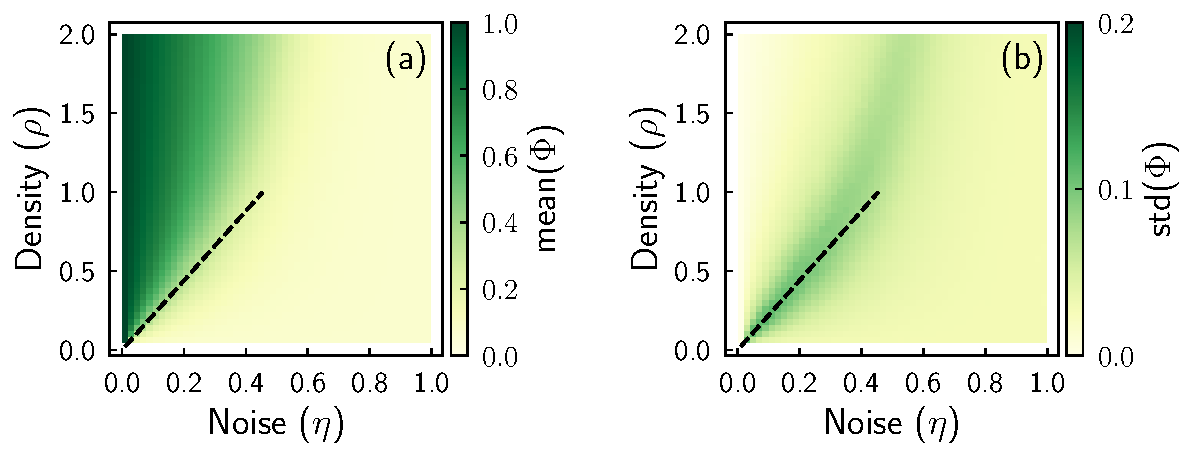
\includegraphics[width=\linewidth]{phase-vicsek}
  \caption[The phase behaviour of the Vicsek model]{
  The phase behaviour of the Vicsek model. The simulation was performed at different state points, with different density and noise values. The total number of states was $50 \times 50 = 2500$. For each state point, 200 agents were simulated, whose speed was fixed at 0.1. The system was updated $2\times10^4$ steps to reach steady state. The polarisation of the system was recorded in the subsequent $2\times10^4$ steps.
  (a) The time-average polarisation at different states.
  (b) The standard deviation of the polarisation at different states. This value represents the susceptibility of the system.
  The dashed line in both subplots indicates a linear relationship between the transitional density and noise. The end of the dashed line \emph{does not} imply the presence of a critical point.
  }
  \label{fig:phase-vicsek}
\end{SCfigure}


The Vicsek model is a very simple active matter model for the dynamics of the animals \cite{vicsek1995}. Essentially, the agents align with nearby neighbours in the model, leading to the ordered movement.
The Vicsek model and its derivatives enjoyed considerable success in describing the collective behaviour of animals. Typically, the equation of motion for the Vicsek model is written as \cite{vicsek1995},

\begin{equation}
\begin{split}
	\mathbf{v}_{i}^{t+1}
	&=
    v_{0} \mathcal{R}_{\eta} \left[\Theta\left(
            \sum_{j \in S_{i}} \mathbf{v}_{j}^t
    \right)\right]
    = \mathcal{V} (\mathbf{v}_{i}^t) \\
	\mathbf{x}_i^{t+1}
	&= \mathbf{x}_i^{t} + \mathbf{v}_i^{t+1},
\end{split}
\label{eq:vicsek}
\end{equation}

\marginpar{
\centering
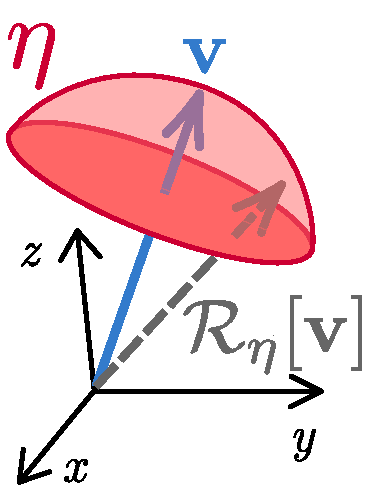
\includegraphics[width=0.7\marginparwidth]{vicsek-noise}
\captionof{figure}{The scalar noise in the Vicsek model.}
}

\noindent where \gls{vit} represents the velocity of the $i$th agent at time point $t$.
The symbol \gls{si} represents the set containing the neighbours of agent $i$ within the unit distance.
The operator \gls{opnorm} is responsible for normalising a vector to unit norm. The operator \gls{oprot} will rotate a vector randomly around its orientation, adding orientational noise into the system. Such random rotation effectively draws a spherical cap around the vector to be rotated, and the value of \gls{eta} determines the area of this spherical cap.
Formally, the noise is referred to as \emph{scalar noise} in the Vicsek model, as opposed to vectorial noise \cite{pimentel2008}.
We use the symbol \gls{opvicsek} to represent the velocity updating rule of the Vicsek model.


The important parameters for the Vicsek model are the noise ($\eta$) and the number density ($\rho$), when we set the interaction range to one. The noise controls the randomness of the system, and the density controls the neighbour set $S_{i}$ for particle $i$. In addition to $\rho$ and $\eta$, another contributing parameter is the speed of the agents ($v_0$ in Eq.~\ref{eq:vicsek}), but its effect is less significant than $\eta$ and $\rho$. Therefore, we will only focus on $\eta$ and $\rho$.



The behaviour of the Vicsek model is presented in Fig.~\ref{fig:phase-vicsek} (a), characterised by the polarisation ($\Phi$) as the order parameter. In the low noise and high density region, the system exhibits ordered behaviour. For the low density and high noise simulations, the agents move randomly with a small $\Phi$ value. Figure~\ref{fig:phase-vicsek} (b) shows the standard deviation of the polarisation from the simulation, whose maximum value indicates the transition between the ordered phase and the disordered phase. In the dilute region, where $\rho < 1$, the transitional density \gls{rhoc} and noise \gls{etac} have a linear relationship, as indicated by the dashed line in Fig.~\ref{fig:phase-vicsek}. Such linear relationship is in accordance with previous 3D numerical simulation results \cite{puzzo2019}.

 

If we try to compare the Vicsek model with the experimental result, the model would fail, as shown in Fig.~\ref{fig:model-dynamics} (a). 
This is because the real zebrafish reached the most random state ($\Phi \sim 0.13$), with a minimum $\kappa$ value of 1.5. That is to say, the fish would have some excess persistence length even in their most random states.
The excess persistence length is expected, as the real fish do not change their orientation at arbitrarily high frequencies. However, this ``minimum persistence length'' does not exist in the Vicsek model, as the Vicsek agents do indeed, change their orientation at a frequency $\sim \infty$, in their most random state, where $\eta = 1$, and $\Phi \sim 0.13$.


\subsection{The Effect of Inertia}
\label{section:model-vicsek-inertia}

\begin{SCfigure}
  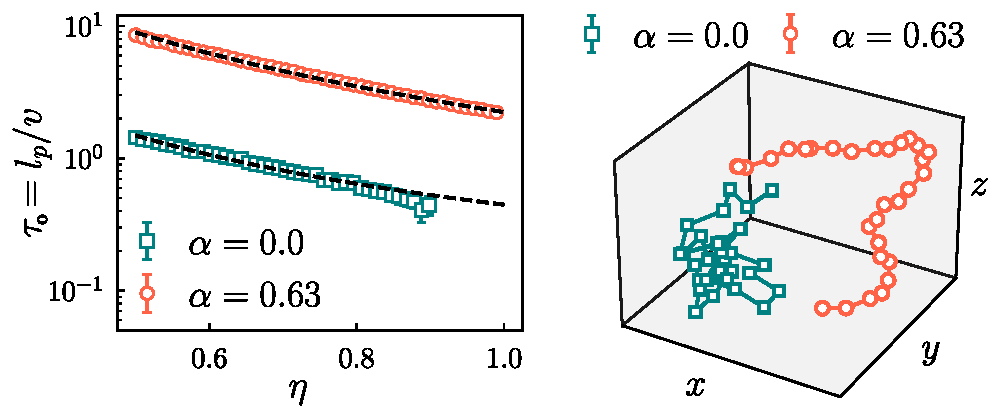
\includegraphics[width=\linewidth]{vicsek-inertia}
  \caption[The effect of inertia in the Vicsek model]{
	The effect of inertia, noted as $\alpha$ in Eq.~\ref{eq:vicsek-inertia}, for a single agent in the Vicsek model.
	(a) The relaxation time of the orientation as a function of the orientation noise ($\eta$). The dashed line shows a polynomial fit, where we assume $\tau_\mathbf{o} \sim \eta^{-2}$ \cite{ginelli2016}. For the Vicsek model in the noisy region ($\eta > 0.9$), the relaxation time is hard to measure because of its small numerical value.
	(b) The trajectories of agents with different $\alpha$ values.
  }
  \label{fig:vicsek-inertia}
\end{SCfigure}


One heuristic approach to modify the Vicsek model, so that the model could fit the experimental result, is to remedy the extreme zigzag movement of the agents in the high noise region. For a real zebrafish, we expect its swimming pattern to be inertial, since the Reynold number for an adult zebrafish is around 20000 \cite{danos2012}. To incorporate an effective inertia, we could simply let the agents to remember their previous orientations, by rewriting the equation of motion as the following,


\begin{equation}
\begin{split}
	\mathbf{v}_{i}^{t+1}
	&= v_0 \Theta \left[
		(1 - \alpha) \mathcal{V}(\mathbf{v}_i^t) +
		\alpha \mathbf{v}_i^t
	\right]
    \\
	\mathbf{x}_i^{t+1}
	&= \mathbf{x}_i^{t} + \mathbf{v}_i^{t+1},
\end{split}
\label{eq:vicsek-inertia}
\end{equation}


\noindent which is effectively a linear mixture of the Vicsek interaction, noted as $\mathcal{V}(\mathbf{v}_i^t)$, and the original velocity ($\mathbf{v}_i^t$).
The parameter \gls{alpha} controls the ratio between the moving direction from Vicsek interaction to the existing moving direction, and we call it the \emph{inertia}.
When $\alpha$ is zero, the model is reduced to the Vicsek model.
When $\alpha$ is one, all the agents will travel ballistically without any interaction. The trajectories of a single agent with different $\alpha$ values are presented in Fig.~\ref{fig:vicsek-inertia}(b). The agent with moderate $\alpha$ value presents a smooth trajectory, as expected.
Figure~\ref{fig:vicsek-inertia} (a) shows the scaling relationship between the orientational relaxation time and the noise, where $\tau_\mathbf{o} \sim \eta^{-2}$. Such relationship is in accordance with previous proposals \cite{ginelli2016, puzzo2019}. The incorporation of the ``inertia'' ($\alpha$) does not change such the scaling relationship, and it only slows down the relaxation of the orientation of the agents.



The behaviour of the Vicsek model with the inertia is shown in Fig.~\ref{fig:phase-vicsek-inertia}. The structure of the phase diagram\marginfootnote{
	Figures~\ref{fig:phase-vicsek-inertia} (a) and (c), as well as Fig.~\ref{fig:phase-vicsek} (a), revealed two phases of the Vicsek model: the ordered phase with high $\Phi$ values, and the disordered phase with $\Phi \sim 0$.
}
is similar to that without inertial, where the agents exhibits ordered behaviour in the high density and low noise region, and they perform random movement in the dilute and noisy states. However, the incorporation of the inertia ($\alpha = 0.63$), visually, increases the area of the ordered region in Fig.~\ref{fig:phase-vicsek-inertia}.
Here we give a hand-waving argument for such an observation. The increase of the $\alpha$ value would increase the persistence length of the agents (Fig.~\ref{fig:vicsek-inertia}). Therefore, these agents would interact with more neighbours, before they forget their original orientations. The increased interaction promotes the propagation of the information within the group, leading to ordered movement.


At a moderate density level ($\rho = 1$), the phase diagram spanned by the noise $\eta$ and the inertia $\alpha$ is presented in Fig.~\ref{fig:phase-vicsek-inertia} (c), with the corresponding susceptibility shown in Fig.~\ref{fig:phase-vicsek-inertia} (d). Generally, the increasing $\alpha$ value expands the ordered region in the parameter space (Fig.~\ref{fig:phase-vicsek-inertia}), which is in accordance with the argument that $\alpha$ increase the order of the system by inducing more interactions among the agents.% The line separating the ordered phase and disordered phase in Fig.~\ref{fig:phase-vicsek-inertia} (d) is more complicated, comparing with the same order-disorder transition line in Fig.~\ref{fig:phase-vicsek-inertia} (b). 

\begin{SCfigure}
  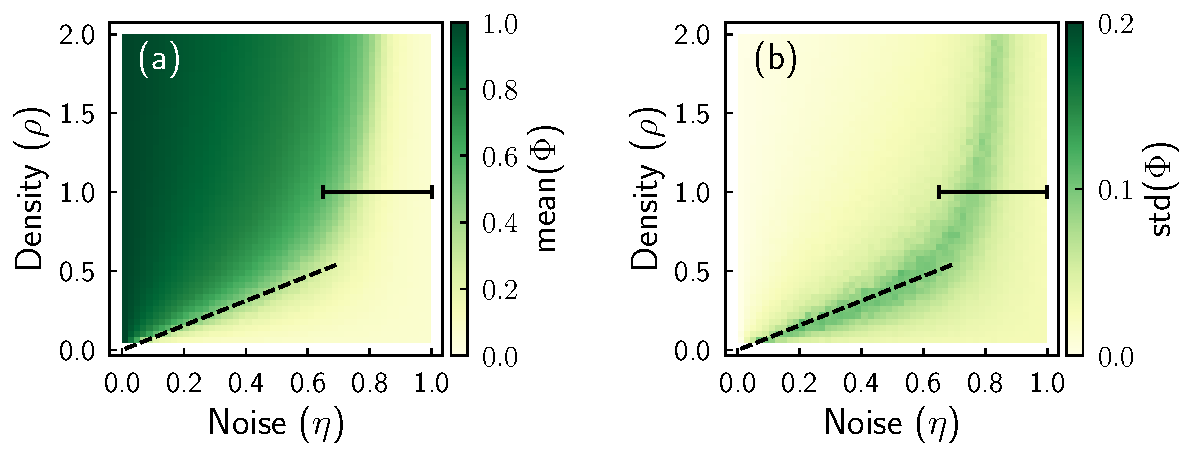
\includegraphics[width=\linewidth]{phase-vicsek-inertia}
  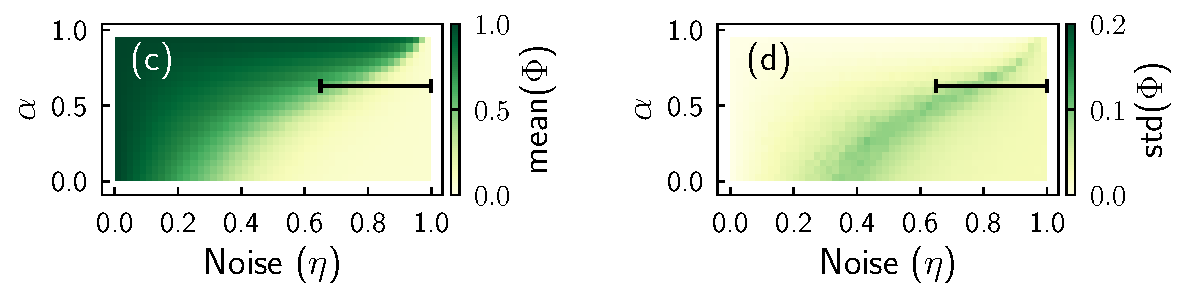
\includegraphics[width=\linewidth]{phase-vicsek-alpha-200}
  \caption[The phase behaviour of the Vicsek model with inertia]{
  The phase behaviour of the Vicsek model with inertia. The simulation detail is the same to those described in Fig.~\ref{fig:phase-vicsek}. The horizontal bars represents the region that matched our experimental results.
  (a) The time-averaged polarisation at different states with different $\rho$ and $\eta$ values, with $\alpha=0.63$.
  (b) The standard deviation of the polarisation at different states with different $\rho$ and $\eta$ values, with $\alpha=0.63$. This value represents the susceptibility of the system.
  (c) The time-averaged polarisation at different states with different $\alpha$ and $\eta$ values, with $\rho=1$.
  (d) The standard deviation of the polarisation at different states with different $\alpha$ and $\eta$ values, with $\rho=1$. This value represents the susceptibility of the system.
  }
  \label{fig:phase-vicsek-inertia}
\end{SCfigure}



\subsection{Comparing with the Experiment}

The parameters in the Vicsek model with inertia, namely the noise $\eta$, the density $\rho$, and the inertia $\alpha$, were manually adjusted to fit the 3D experimental observations in section~\ref{section:universal}. The comparison was shown in Fig~\ref{fig:model-dynamics} (a), where the simulation results were plotted as a solid line, and it matches the experimental results. This line was obtained by simulating the Vicsek model with a fixed speed ($v = 0.1$) and fixed inertia ($\alpha=0.63$), while varying the value of the noise term ($0.65 \le \eta \le 1$). The parameters being simulated were also plotted as horizontal bars in Fig.~\ref{fig:phase-vicsek-inertia}.

The matching between the simulation and the experimental results indicates the existence of effective alignment between the fish. And the increasing persistence length at fixed nearest neighbour distance promotes the transformation of information in the group, therefore increase the order. 

We also calculated the connected correlation function ($C_\mathbf{o}(r)$, Eq.~\ref{eq:cr}) of the orientation for the simulation results, and compared the results with the one in the simulation. The comparisons were plotted in Fig.~\ref{fig:model-dynamics} (b) and (c). In Fig.~\ref{fig:model-dynamics} (b), the correlation function from the states with a low $\kappa$ value were compared, and the results in Fig.~\ref{fig:model-dynamics} (c) shows the correlation function in the states with high $\kappa$ values. In both cases, the simulated agents exhibits different $C_\mathbf{o}(r)$, compared with the zebrafish. Such deviation is expected, as the information about the spatial correlations, like the $g(r)$, was ignored in our model.

\begin{SCfigure}
  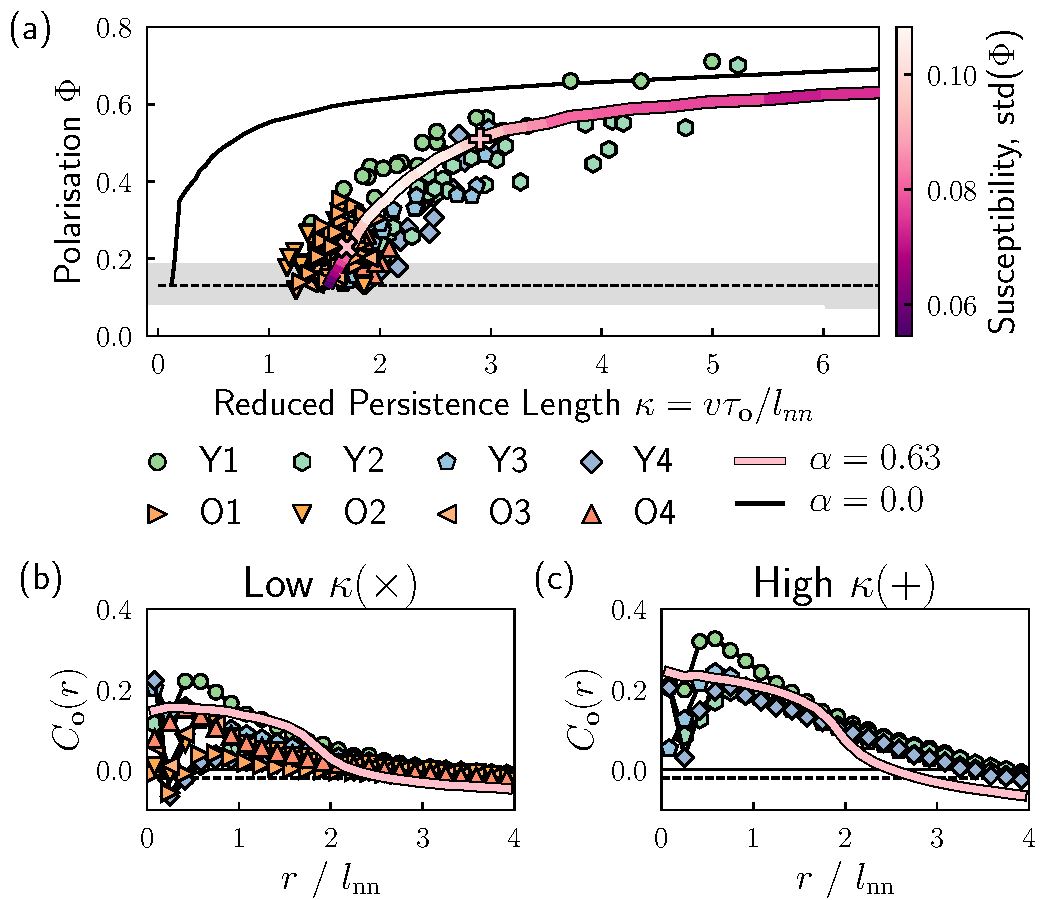
\includegraphics[width=\linewidth]{model-dynamics}
  \caption[Comparing the dynamics of the zebrafish with the Vicsek model simulation]{
  Comparing the dynamics of the zebrafish with the Vicsek model simulation.
  (a) The relationship between the rescaled persistence length $\kappa$ and the polarisation $\Phi$. The scatters represent different experimental observations. The solid line represent the simulation result with Vicsek model ($v=0.1, \alpha=0, \rho=1, 0.18 \le \eta \le 0.9$). The thick solid line with colour represent the simulation result of the Vicsek model with inertia ($v=0.1, \alpha=0.63, \rho=1, 0.65 \le \eta \le 1$). The brightness of the colour represent the standard deviation of the polarisation in different states.
  (b) The connected correlation function $C_\mathbf{o}(r)$, calculated from the experimental data (scatters) and the simulation (solid line) in the low $\kappa$ region.
  (c) The connected correlation function $C_\mathbf{o}(r)$, calculated from the experimental data (scatters) and the simulation (solid line) in the high $\kappa$ region.
  }
  \label{fig:model-dynamics}
\end{SCfigure}

Our model for the dynamics of the fish revealed the importance of the inertia. As mentioned in section~\ref{section:vicsek-model} and shown in Fig.~\ref{fig:model-dynamics} (a), the Vicsek model without inertia, whose $\alpha$ value equals zero, could not fit the experimental result. The mismatch between the model is especially significant in the low $\kappa$ region where the noise term is high, which is related to the unrealistic zig-zag movement of the Vicsek agents (Fig.~\ref{fig:vicsek-inertia}). The increasing of the $\alpha$ value shifted the simulation result to the high $\kappa$ region, that matches the experimental result.


The simplicity of our model is important. The good fit between the simulation results and the experimental results indicates that the order of the dynamics (the polarisation) for the zebrafish group can be described the four parameters (the density, the inertia, the speed, and the noise) in the model. This is because the dynamics of the fish group is dominated by their effective alignment interaction. For a group of 50 fish, their changing states can be captured by the noise parameter ($\eta$ in Eq.~\ref{eq:vicsek}), as shown in Fig.~\ref{fig:model-dynamics} (a), suggesting the observed zebrafish behaviour is universal.


It is also important to point out that our model suggests that the fish were effectively crossing the between the ordered phase and the disordered phase (see the horizontal bars in Fig.~\ref{fig:phase-vicsek-inertia}). The location of the boundary, for 50 agents, is located at $\kappa \sim 2$, where the susceptibility of the polarisation took its maximum, as shown in Fig.~\ref{fig:model-dynamics} (a).
This result is expected for the collective behaviour from a group of animals. Sometimes it is referred to as a dogma that ``all biological systems were poised near a critical state'' \cite{mora2011}. For the observed fish, they were clearly not just staying at a critical state, because the state of the group was constantly changing (section~\ref{section:change-states-2d} and \ref{section:change-states-3d}). However, the simulation indicates that the fish were, at least, close to the phase boundary between the ordered movement and disordered. In other words, the animals tend to stay on the fence, between the ordered state and the disordered state.
Such choice is understandably beneficial, because staying in the disordered state essentially means the group could not move collectively. On the other hand, forcing the group in the ordered state means the informed individual could not change the overall moving direction of the entire group.

\subsection{Limitations of the Model}

Finally, it is important to address the several limitations of our simulation, even though the fitting is visually good. First of all, the agents in the Vicsek model have a constant speed ($v$ in Eq.~\ref{eq:vicsek}), and this is different from the zebrafish. In addition, the only interaction between the agents is the alignment, while we could see evidence for the repulsive interaction and attractive interaction amongst the fish in section~\ref{section:analysis-structure-2d} and \ref{section:analysis-structure-3d}. Finally, the inhomogeneity of the density inside the tank is ignored in the Vicsek model, and the agents was enclosed in a periodic boundary, rather than a fish tank.

\vfill
\pagebreak

\begin{adjustwidth}{0cm}{-5cm}
\begin{tcolorbox}[
title=Summary of Chapter~6,
fonttitle=\sffamily\Large,
right=0.1\linewidth,
enlarge bottom by=0.5em,
enlarge top by=0.5em,
]
\begin{itemize}
	\item We modelled the density distribution of the fish as an equilibrium system, featuring the following elements.

	\begin{itemize}
		\item The observation tank as a hard boundary.
		\item The depth preference of the fish as an effective gravity.
		\item The holes on the tank which repel the fish.
		\item The fish-fish interaction inferred from the $g(r)$ of the fish.
	\end{itemize}

	\item By fitting the experimental density distribution and the results from the model, we get the following conclusions.
	\begin{itemize}
		\item For the 1/2/3 fish experiments, the interaction between the fish and the environment dominates the density distribution.
		\item For a group of 50 zebrafish, the fish-fish interaction is important to their density distribution.
	\end{itemize}
	
	\item We modelled the ordering process of the dynamics of the fish group with an active matter model (the Vicsek model). We get the following results.
	\begin{itemize}
		\item The original Vicsek model can not fit the experimental data.
		\item If an inertia term was added to the Vicsek model, the simulation results fit the experimental data.
		\item The universal relationship between the reduced persistence length ($\kappa$) and the polarisation ($\Phi$) reported in section~\ref{section:universal} can be understood, as the decreasing noise ($\eta$) values in our model, which lead to higher polarisation.
	\end{itemize}
	\item There are several limitations for our model.
	\begin{itemize}
		\item  The simulations carried out in section~\ref{section:simulate-density}, to model the density distribution of the fish, ignored the dynamics of the system, by assuming the density profile was from an equilibrium system.
		\item The simulations in section~\ref{section:simulate-dynamics}, to model the dynamics of the fish, ignored the inhomogeneous density distribution, as well as the two point density correlation observed from the experimental $g(r)$ profile.
	\end{itemize}
\end{itemize}
\end{tcolorbox}
\end{adjustwidth}
%
%\newpage
%
%\section{Summary}
%
%In this chapter we modelled the 3D behaviour of the zebrafish, in order to get more insights from the experimental data. In section~\ref{section:simulate-density}, the density distribution of the fish were modelled as an equilibrium system, with interacting agents, under an external field. Our model indicates that the distribution of the fish was affected by the boundary, the gravity, and the holes drilled on the tank. In addition, the fish-fish interaction also contributes significantly to the density distribution for a large group of fish.
%
%In section~\ref{section:simulate-dynamics}, we matched our result with the Vicsek model. To fit the experimental data, an extra inertia term had to be incorporated to the model. The fitting between the model and the observation gives an explanation for the universal relationship between the reduced persistence length ($\kappa$) and the polarisation ($\Phi$) reported in section~\ref{section:universal}. Typically, the increasing value of $\kappa$ corresponds to the increased interaction among the fish, which could be mapped to decreasing noise ($\eta$) values in our model. In other words, the interaction among the zebrafish leads to, effectively, Vicsek-like alignment. As a result, the entire group would exchange information about the orientation effectively at larger $\kappa$ value, forming the ordered movement.
%
%
%It is important to emphasise the limitation of the models in this chapter. The simulation carried out in section~\ref{section:simulate-density} ignored the dynamics of the system, by assuming the density profile was from an equilibrium system. On the other hand, the simulation in section~\ref{section:simulate-dynamics} ignored the inhomogeneous density distribution, as well as the two point density correlation observed from the experimental $g(r)$ profile. In both cases, the underlying assumptions were crude. To put the two pieces together, and recover a more realistic model for the fish, we could incorporate the non-equilibrium nature of the active matter into the Monte-Carlo simulation, following the new simulation technique from \citeauthor{klamser2021} \cite{klamser2018, klamser2021}. It is also possible to incorporation the external effect into the dynamical simulation \cite{couzin2002, gautrais2012}, making it more realistic. Alternatively, the continuum models of active matter \cite{toner1995, solon2015} may also help explaining the observed results.

\end{document}
